% % % Set the style for this file:
\pagestyle{standard}

% % % Beginning of the chapter
\chapter{Notions of infrared thermography}\label{chapter1}

	% % % Set the style for the first page:
	\thispagestyle{chapter-first-page}
	
	\section{Infrared radiation spectrum.}\label{section1.1}
	
		Infrared (IR) radiation is the energy irradiated by a surface that has a temperature above the absolute zero [1]. Within the electromagnetic spectrum, IR radiation is defined as the radiation band that spans from 0.7 $\mu$m to 1000 $\mu$m in wavelength (Figure \ref{fig1.1}).
		
		Much of the IR spectrum, however, is not useful for Infrared thermography (IRT) due to atmospheric absorption. This absorption occurs mainly with $H_{2}O$ and $CO_{2}$ molecules as they are well known for being good heat absorbers (Figure \ref{fig1.2}). According to this fact, the IR wavelength range is sometimes further divided into 4 additional categories:

		\begin{enumerate}[label={\Roman*.}]
			\item Near-infrared (NIR) from 0.8 $\mu$m to 1.7 $\mu$m.
			\item Short-wavelength infrared (SWIR) from 1 $\mu$m to 2.5 $\mu$m.
			\item Mid-wavelength infrared (MWIR) from 2 $\mu$mm to 5 $\mu$mm.
			\item Long-wavelength infrared (LWIR) from 8 $\mu$mm to 14 $\mu$mm.
		\end{enumerate}
		
		\begin{figure}[ht!]
			\centering
			\captionsetup{justification=centering,margin=2cm}
			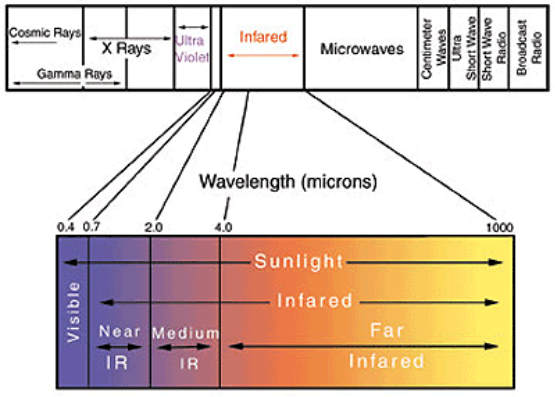
\includegraphics[scale=0.75]{Figures/Chapter01/lightspectrum}
			\caption{Electromagnetic spectrum showing the portion corresponding to IR radiation.}\label{fig1.1}
		\end{figure}
		
		It is important to note that this classification is somewhat arbitrary and therefore it can change quite a bit from one author to the other but in general they remain fairly similar. Most IR sensors are designed to work in the LWIR part of the spectrum since this is the range that minimizes this absorptions.
		
		In this study, as we use an IR camera sensitive only to the fourth type, we will refer to IR as the LWIR except otherwise explicitly stated.
		
		\begin{figure}[ht!]
			\centering
			\captionsetup{justification=centering,margin=2cm}
			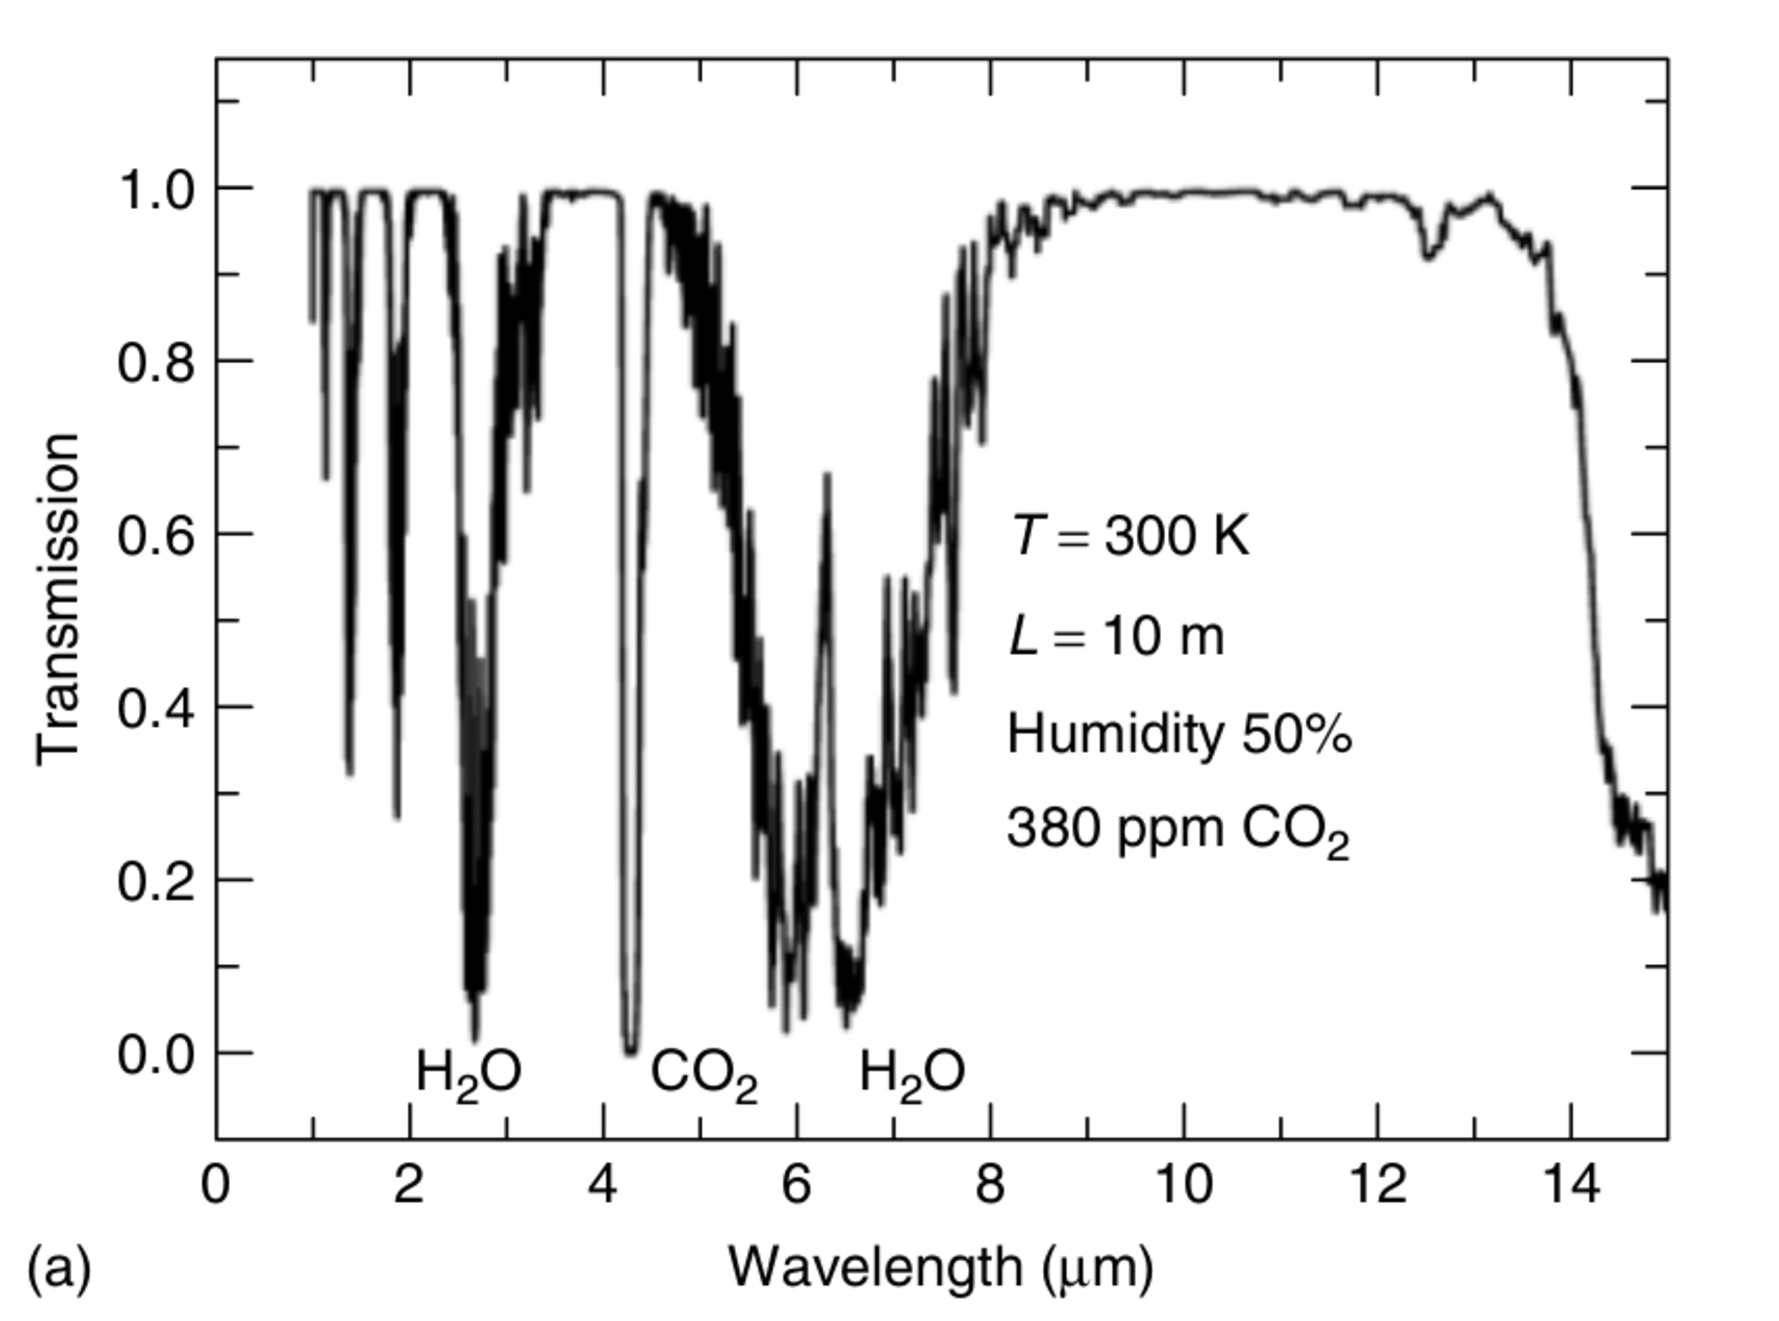
\includegraphics[scale=0.45]{Figures/Chapter01/Transmission.pdf}
			\caption{A typical atmospheric transmittance plot  for infrared radiation. For some of the minima we can see the absorbing molecule responsible.}\label{fig1.2}
		\end{figure}
		
	\section{Plank's law for blackbodies. IR radiation dissipation.}\label{section1.2}
	
		According to Plank's law, the IR emissive power of a blackbody at a temperature $T$, with a wavelength between $\lambda$ and $\lambda+d\lambda$ is given by Equation \ref{eq1.1}, where $C_{1}$ and $C_{2}$ are constants, often called first and second radiation constants respectively [2].
		
		\begin{equation}\label{eq1.1}
			N_{b}(\lambda,T)d\lambda=\frac{C_{1} \cdot \lambda^{-5}}{\exp (\frac{C_{2}}{\lambda\cdot T}) -1} d\lambda
		\end{equation}
		
		Figure \ref{fig1.3} shows this functional dependence for six different temperatures [3]. The gray line represents the displacement of the maximum for each temperature. Note that, as the temperature decreases, the maximum emissive power moves to higher wavelengths, this is known as the Wien's displacement law [4]. 
		
		There are three ways by which the emissive power striking an object may be dissipated: absorption, transmission and reflection [5]. The fractions of the total radiant energy that are associated with each of these modes of dissipation are referred to as the \textit{absorptivity}, \textit{transmissivity} and \textit{reflectivity} of the body. Three parameters are used to describe these phenomena: the spectral \textit{absorptance} $\alpha$, which is the fraction of the spectral emissive power absorbed by the object, the spectral \textit{reflectance} $\rho$, which is the fraction of the spectral emissive power reflected by the object, and the spectral \textit{transmittance} $\tau$, which is the fraction of the spectral emissive power transmitted by the object.
		
		\begin{figure}[ht!]
			\centering
			\captionsetup{justification=centering,margin=2cm}
			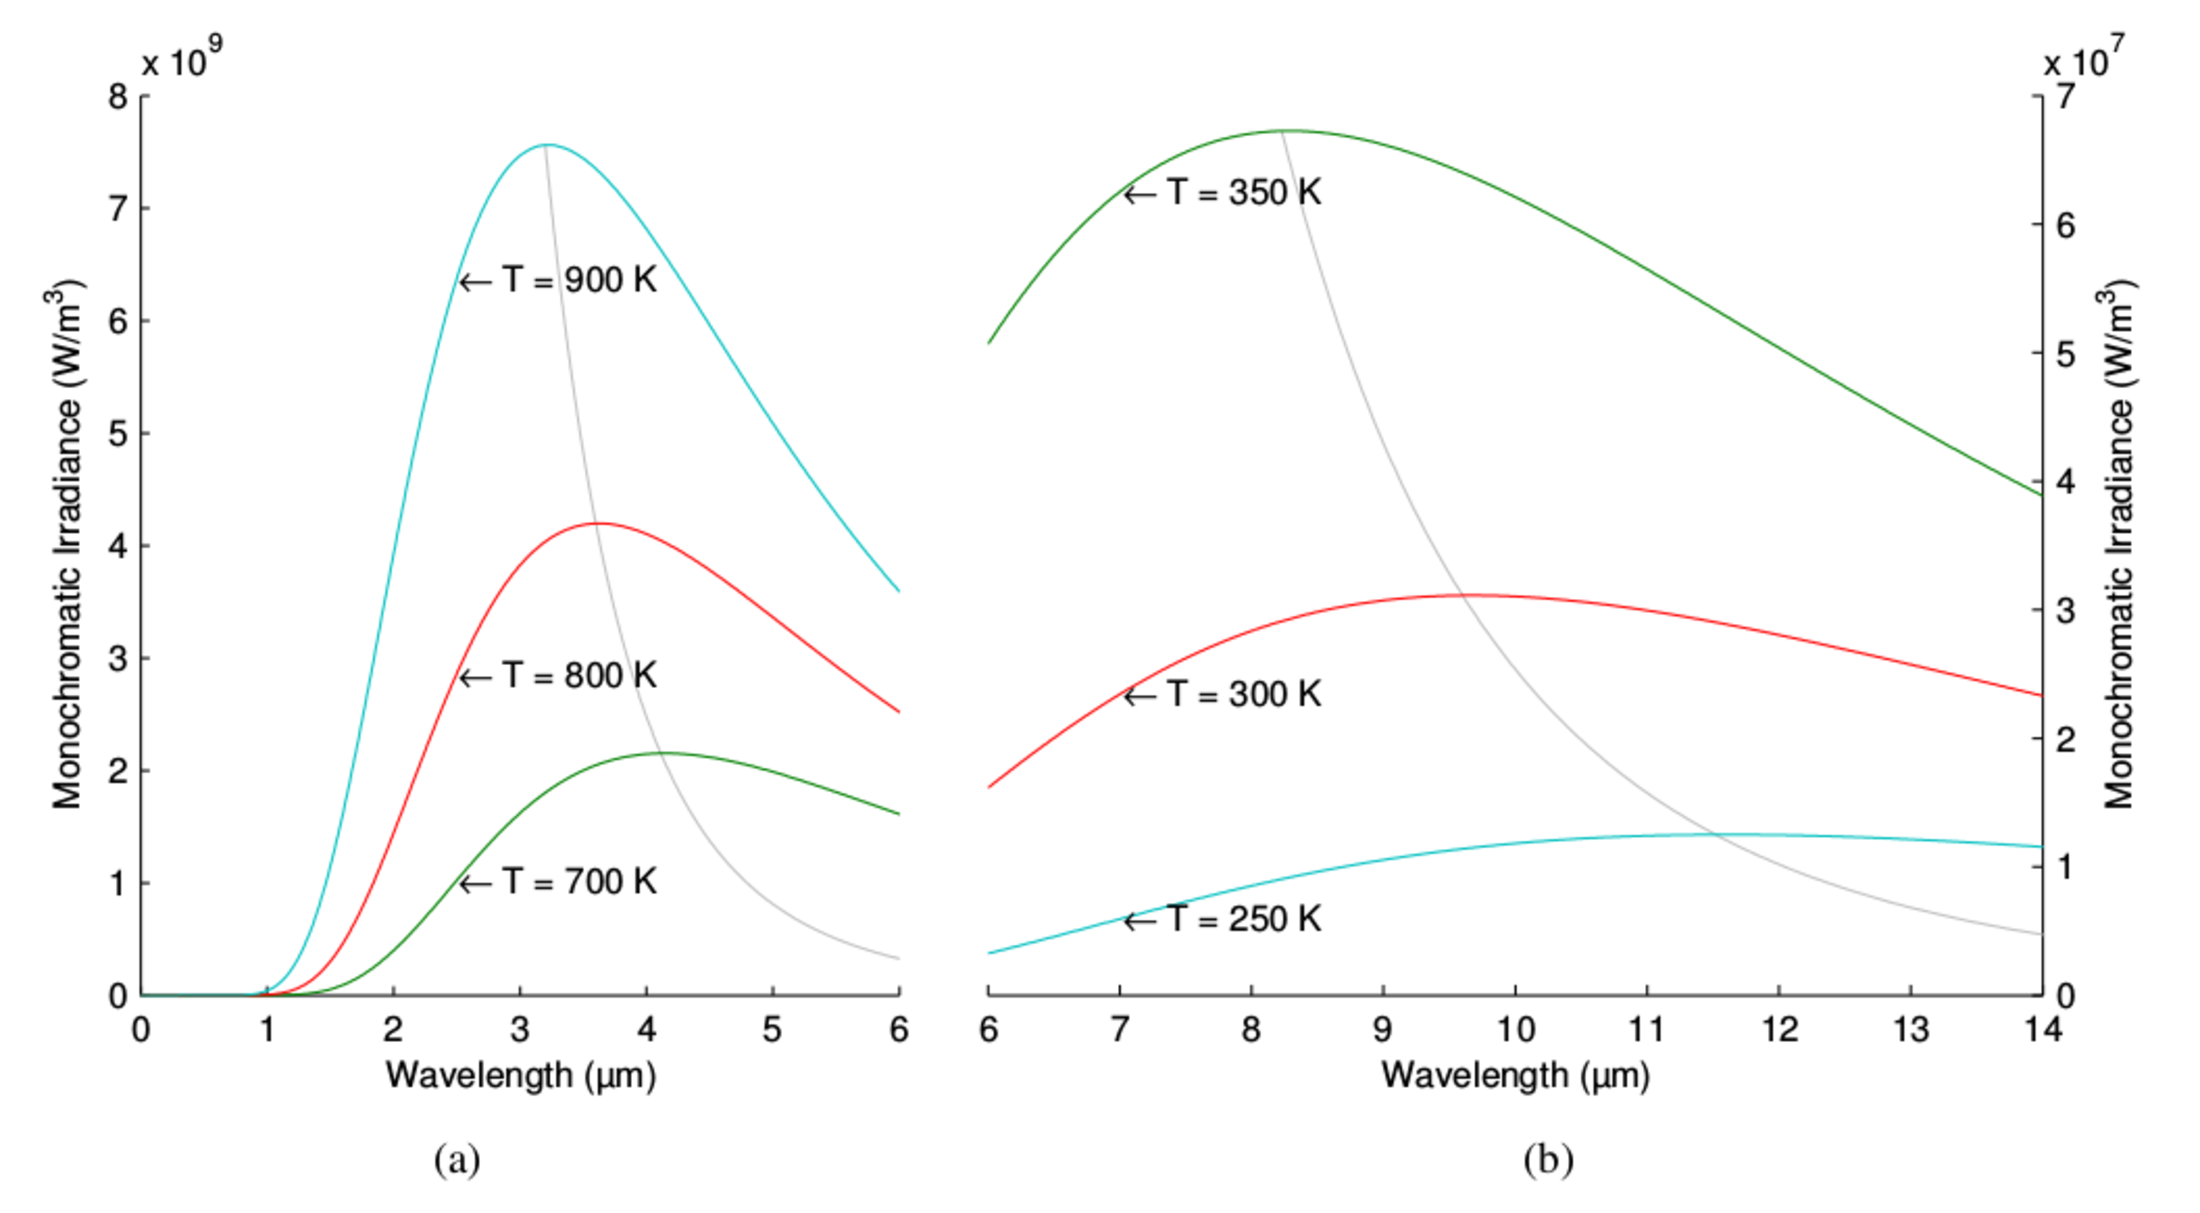
\includegraphics[scale=0.45]{Figures/Chapter01/PlankFunction.pdf}
			\caption{Planck's law: electromagnetic radiation emitted by a blackbody in thermal equilibrium at a definite  temperature. (a) Objects with a high temperature emit most of the radiation in the middle wave infrared; (b) Objects with a low temperature emit most of the radiation in the long wave infrared. The two parts of the graph are scaled differently on the y-axis.}\label{fig1.3}
		\end{figure}		
		
		These three parameters are, in general, wavelength dependent and their sum must be one at any given wavelength and surface temperature:
		
		\begin{equation}\label{eq1.2}
			\alpha + \rho + \tau = 1
		\end{equation}
		
		If we regard the surface as \textit{opaque}, it means that the transmission coefficient is $\tau \equiv 0$ and then we can rewrite Equation \ref{eq1.2} as:	
		
		\begin{equation}\label{eq1.3}
			\alpha + \rho + \tau = 1
		\end{equation}
		
	\section{Emissivity definition. Kirchhoff's law.}\label{section1.3}
		
		One of the most important concepts in IRT is \textit{emissivity}. Emissivity ($\varepsilon$) of a surface at a temperature $T$ for a given wavelength $\lambda$ is defined as the ratio of the emissive power of a  non-blackbody to the emissive power of a blackbody at the same temperature:
		
		\begin{equation}\label{eq1.4}
			\varepsilon(\lambda,T)=\frac{N(\lambda,T)}{N_{b}(\lambda,T)}
		\end{equation}
		
		As the emissivity of a real surface typically ranges between 0 and 1, this relationship tells us that real body emits only a fraction of the thermal energy emitted by a blackbody at the same temperature (Figure \ref{fig1.4}). If the emissivity is constant and independent of the wavelength, the body is called a \textit{greybody}.
		
		\begin{figure}[ht!]
			\centering
			\captionsetup{justification=centering,margin=2cm}
			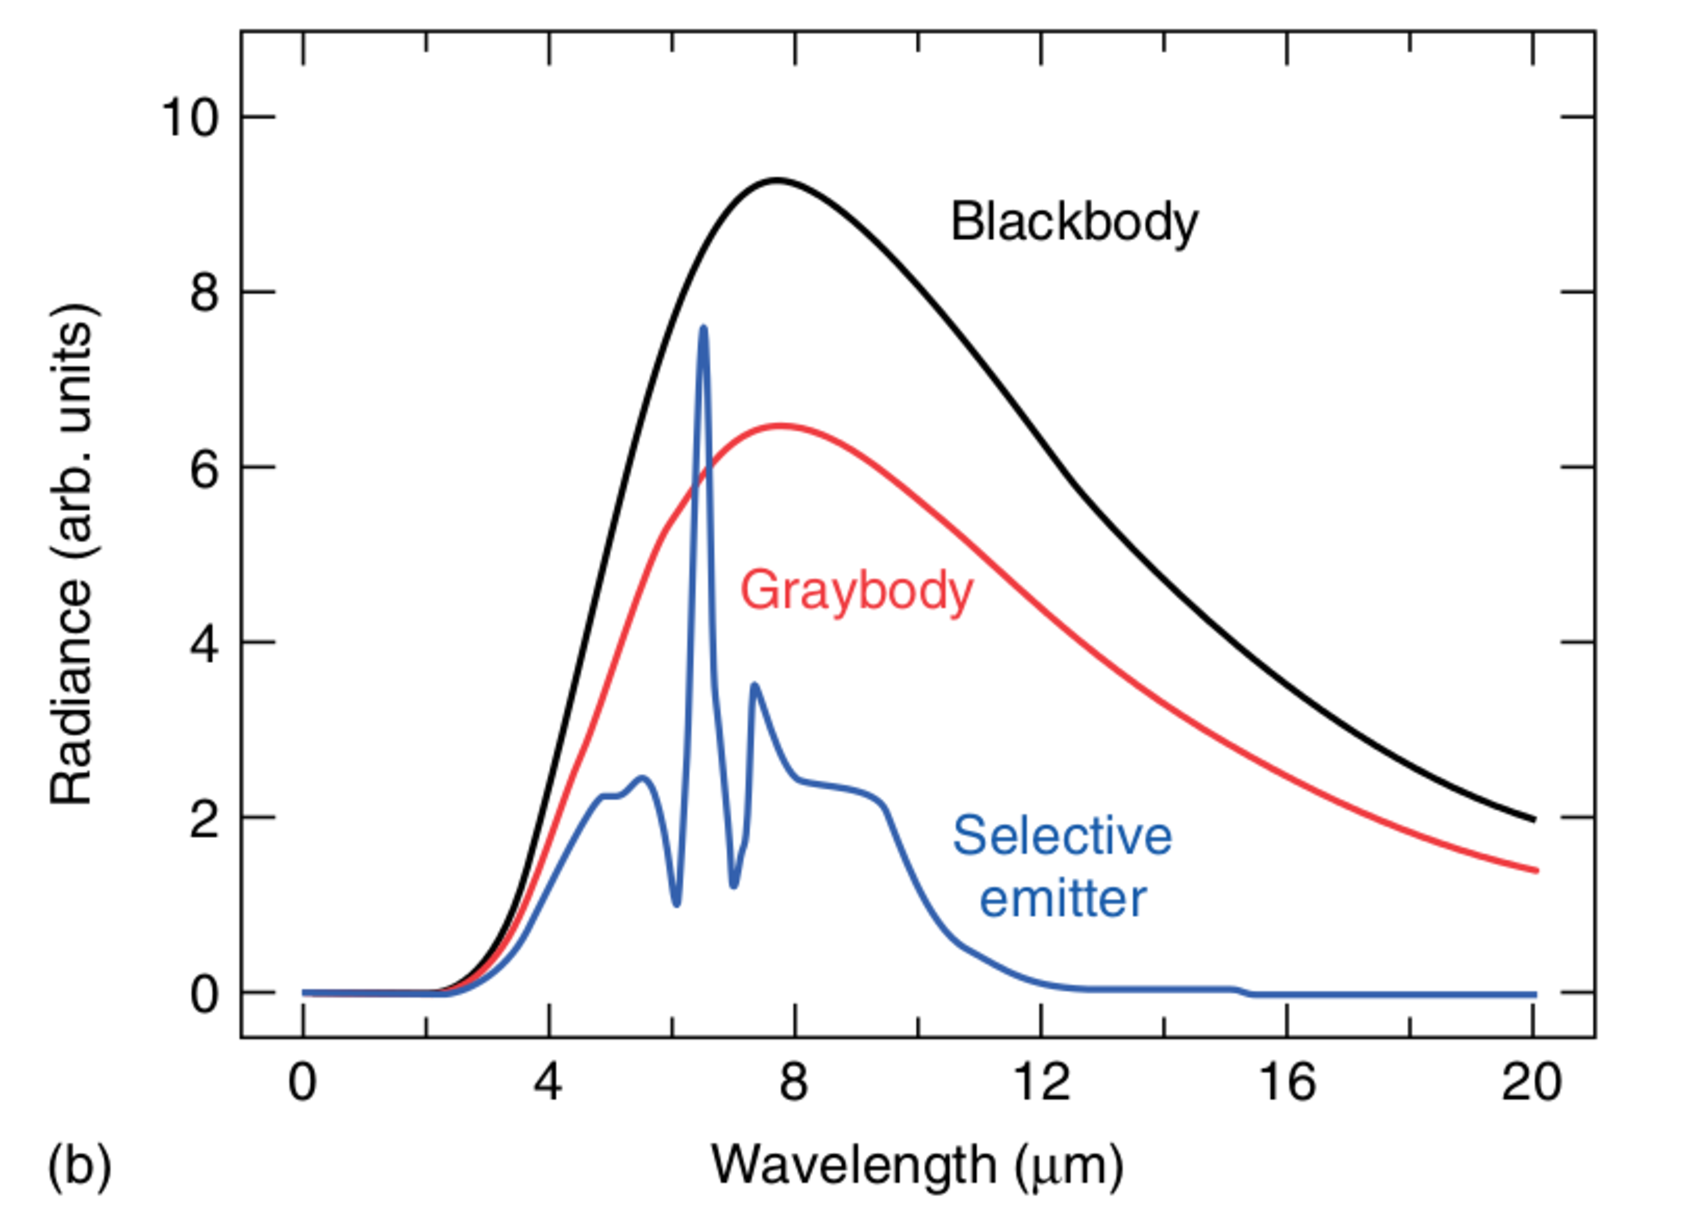
\includegraphics[scale=0.45]{Figures/Chapter01/BlackAndGreybodyComparison.pdf}
			\caption{Relationship between the blackbody spectral radiation and the radiation emitted by a greybody and a selective radiator at the same temperature. It can be seen how the blackbody yields the maximum radiance at any given wavelength due to the value of $\varepsilon=1$.}\label{fig1.4}
		\end{figure}
		
		\bigskip
		The emissivity of real objects, however, is not constant nor independent of the wavelength and therefore they cannot be considered greybodies. In fact, it might also depend on many other factors such as temperature and viewing angle, as we will discuss later. However, it is usually assumed that for short wavelength intervals, the emissivity can be considered as a constant. This assumption is used to treat real objects as greybodies in order to avoid the associated mathematical complications of emissivity estimation. For this reason, surface emissivities are often computed as the average of the emissivity through the wavelength interval in which the infrared sensor works. This average is also possible because the emissivity is a slow-varying function of wavelength for solid objects. However, this does not apply to other cases, such as gases or liquids.
		
		The blackbody, as a perfect emitter, will have an emissivity of 1 while non-blackbodies will have, as mentioned earlier, emissivity values in the range $0<\varepsilon<1$. If a blackbody is surrounded by an isothermal black enclosure of the same temperature, then in thermodynamic equilibrium, such blackbody will have to absorb 100\% of the radiation emitted by the enclosure. At the same time it will emit 100\% of its own thermal radiation since it has $\varepsilon=1$. Under those circumstances, the following relationship holds:
		
		\begin{equation}\label{eq1.5}
			\alpha \equiv \varepsilon=1
		\end{equation}	
		
		This is known as the Kirchhoff's law (for the blackbody). In general for non-blackbodies, according to this law, the emissivity and absorptivity of any material are equal at any specified temperature and wavelength. Thus, we can rewrite Equation \ref{eq1.2} as:	
		
		\begin{equation}\label{eq1.6}
			\varepsilon + \rho + \tau = 1
		\end{equation}	
		
		And for the case in which $\tau=0$, this becomes:
		
		\begin{equation}\label{eq1.7}
			\varepsilon = 1 - \rho
		\end{equation}	
		
		
			